% oe.tex — الزوجي والفردي
% Compile with: xelatex oe.tex
% قفل: Def. 0.0 — S مضغوطة، S(n) فردي دائماً.
\documentclass[12pt,a4paper]{article}
\usepackage{polyglossia}
\setmainlanguage{arabic}
\setotherlanguage{english}
\setmainfont{Amiri}
\newfontfamily\englishfont{Amiri}
\usepackage{amsmath,amssymb,amsthm}
\usepackage{booktabs}
\usepackage{hyperref}
\usepackage{xcolor}
\usepackage{graphicx}
\usepackage{fancyhdr}
\usepackage{lastpage}
\definecolor{gold}{HTML}{B48A00}

\theoremstyle{definition}
\newtheorem{definition}{تعريف}[section]
\newtheorem{example}{مثال}[section]
\theoremstyle{plain}
\newtheorem{lemma}{لمّة}[section]
\newtheorem{theorem}{مبرهنة}[section]
\newtheorem{remark}{ملاحظة}[section]

% ===== الفوتر =====
\pagestyle{fancy}
\fancyhf{}
\fancyhead[L]{\small الزوجي والفردي --- OE}
\fancyhead[R]{\small عبدالله محمد ناصر الجبري}
\fancyfoot[C]{\small تعز - اليمن | jabri-com.vercel.app | صفحة \thepage\ من \pageref{LastPage}}
\renewcommand{\headrulewidth}{0.4pt}
\renewcommand{\footrulewidth}{0.4pt}

% ===== الاسم الكامل والعنوان والبريد - من footer.html =====
\title{الزوجي والفردي \\ \textenglish{Odd-Even --- OE}}
\author{م/ عبدالله محمد ناصر الجبري \\[4pt]
\small تعز - الجمهورية اليمنية \\[2pt]
\small \textenglish{Email: jabri62018@gmail.com} \\[2pt]
\small \textenglish{ORCID: 0009-0003-3319-3822} \\[2pt]
\small \textenglish{Website: jabri-com.vercel.app} \\[2pt]
\small \textenglish{Zenodo: doi.org/10.5281/zenodo.23303899 (v5.0.1)}}
\date{\today}

\newcommand{\nuTwo}{\nu_2}
\newcommand{\compS}{S}

\begin{document}
\maketitle

\begin{center}
\small
\textbf{قفل الترميز --- Def.\ 0.0} \\
$S$ مضغوطة بالكامل: نقسم على كل قوى $2$ دفعة واحدة.
ناتج $S$ دائماً فردي.
\end{center}

\section{التعريف}

\begin{definition}[الدالة المضغوطة $S$]
لكل $n \geq 1$ صحيح، نعرّف $\nuTwo(n)$ بأنه أكبر $k \geq 0$ بحيث $2^k \mid n$.
\[
\compS(n) =
\begin{cases}
\dfrac{n}{2^{\nuTwo(n)}} & \text{إذا كان $n$ زوجياً،} \\[8pt]
\dfrac{3n+1}{2^{\nuTwo(3n+1)}} & \text{إذا كان $n$ فردياً.}
\end{cases}
\]
\end{definition}

\begin{remark}
هذا ليس تعريف كولاتز الخام $f(n)=3n+1$ أو $n/2$.
الخلط بين الخام والمضغوط هو الخطأ الذي صُحّح في هذا الملف.
المثال المرفوض سابقاً $16 \leftarrow 5$ صحيح خاماً لأن $3\cdot 5+1=16$،
لكنه مرفوض تحت $S$ لأن $\compS(5)=1$ وليس $16$.
\end{remark}

\section{لمّات أساسية}

\begin{lemma}[الناتج فردي دائماً]
لكل $n \geq 1$، $\compS(n)$ فردي.
\end{lemma}
\begin{proof}
إذا كان $n$ زوجياً، فقسمنا على $2^{\nuTwo(n)}$، وهي أكبر قوة $2$ تقسم $n$،
فيبقى الجزء الفردي من $n$.
وإذا كان $n$ فردياً، فـ $3n+1$ زوجي، وقسمنا على أكبر قوة $2$ تقسمه،
فيبقى جزؤه الفردي.
\end{proof}

\begin{lemma}[الأبناء الزوجيون]
لكل $m \geq 1$ وكل $k \geq 1$:
\[
\compS(2^k m) = \text{الجزء الفردي من } m.
\]
وبالأخص، إذا كان $m$ فردياً فإن $\compS(2^k m)=m$ لكل $k \geq 1$.
\end{lemma}
\begin{proof}
$2^k m$ له نفس الجزء الفردي الذي لـ $m$، لأن الضرب في $2^k$ لا يغيّر الجزء الفردي.
و$\compS$ للعدد الزوجي هو جزؤه الفردي بالتعريف.
\end{proof}

\begin{lemma}[الأبناء الفرديون]
ليكن $m$ فردياً. عندها $c$ فردي يحقق $\compS(c)=m$ إذا وفقط إذا وُجد $k \geq 1$ بحيث
\[
c = \frac{2^k m - 1}{3}, \qquad (2^k m - 1) \bmod 3 = 0.
\]
\end{lemma}
\begin{proof}
إذا كان $c$ فردياً و$\compS(c)=m$، فبالتعريف $(3c+1)/2^{\nuTwo(3c+1)}=m$،
أي $3c+1 = m \cdot 2^k$ حيث $k=\nuTwo(3c+1)$، ومنه $c=(2^k m-1)/3$.
والعكس: إذا تحقق الشرط، وكان $m$ فردياً، فإن $3c+1=m\cdot 2^k$،
و$\nuTwo(3c+1)=k$ لأن $m$ فردي، فيكون $\compS(c)=m$.
\end{proof}

\begin{theorem}[المعكوس الكامل $S^{-1}$]
\[
\compS^{-1}(m) =
\begin{cases}
\{2^k m \mid k \geq 1\} \cup
\left\{\dfrac{2^k m -1}{3} \;\middle|\; (2^k m -1)\bmod 3 = 0\right\}
& \text{إذا كان $m$ فردياً،} \\[10pt]
\emptyset & \text{إذا كان $m$ زوجياً.}
\end{cases}
\]
\end{theorem}
\begin{proof}
من لمّة الناتج الفردي، لا يوجد أي $c$ يحقق $\compS(c)=m$ إذا كان $m$ زوجياً،
فالمعكوس فارغ.
وإذا كان $m$ فردياً، فالأبناء ينقسمون إلى زوجيين وفرديين:
الزوجيون هم $2^k m$ باللمّة الثانية، والفرديون هم بالصيغة باللمّة الثالثة.
\end{proof}

\begin{remark}[الحلقة الذاتية عند $m=1$]
صيغة الأبناء الفرديين تعطي عند $m=1$ و$k=2$ القيمة $c=1$، لأن $\compS(1)=1$.
هذه حلقة ذاتية، وليست فرعاً جديداً في الشجرة، لذلك تستبعدها الخوارزمية بشرط $c \ne m$.
\end{remark}

\begin{remark}[الزوجي ورقة]
في شجرة $S$، كل عدد زوجي ورقة بلا أبناء، لأن لا أحد يصعد إليه.
الأبناء موجودون فقط للعقد الفردية.
هذا ليس نقصاً في الشجرة، بل نتيجة مباشرة من كون $S$ ناتجها فردي.
\end{remark}

\section{أمثلة متحقق منها}

\begin{example}[$m=5$]
\[
\compS(3)=\frac{10}{2}=5, \quad
\compS(10)=\frac{10}{2}=5, \quad
\compS(13)=\frac{40}{8}=5.
\]
فـ $3$ و$10$ و$13$ كلها أبناء لـ $5$ تحت $S$.
\end{example}

\begin{example}[$m=1$]
أبناء $1$ يشملون:
\[
2,\ 4,\ 8,\ 16,\ 5,\ 21,\ 85,\ \dots
\]
وتحقق: $\compS(5)=1$، $\compS(21)=64/64=1$، $\compS(85)=256/256=1$.
\end{example}

\begin{example}[مسار $27$ تحت $S$]
\[
27 \to 41 \to 31 \to 47 \to 71 \to 107 \to 161 \to 121 \to 91 \to 137 \to 103 \to 155 \to 233 \to 175 \to 263 \to 395 \to 593 \to 445 \to 167 \to 251 \to 377 \to 283 \to 425 \to 319 \to 479 \to 719 \to 1079 \to 1619 \to 2429 \to 911 \to 1367 \to 2051 \to 3077 \to 577 \to 433 \to 325 \to 61 \to 23 \to 35 \to 53 \to 5 \to 1.
\]
\end{example}

\section{الخوارزمية}

\begin{verbatim}
nu2(x):
    k = 0
    while x even:
        x = x / 2
        k = k + 1
    return k

S(n):
    if n even: return n / 2^nu2(n)
    else:      return (3*n+1) / 2^nu2(3*n+1)

children(m):
    if m even: return []          # ورقة، بلا أبناء
    c = [2^k * m for k = 1..K]    # أبناء زوجيون
    for k = 1..K:
        num = 2^k * m - 1
        if num mod 3 == 0:
            d = num / 3
            if d odd and d != m:
                add d               # أبناء فرديون
    return c
\end{verbatim}

\section{جدول القفل}

\begin{center}
\begin{tabular}{lll}
\toprule
الرمز & الشرط & النتيجة \\
\midrule
$S(n)=n/2^{\nuTwo(n)}$ & $n$ زوجي & الجزء الفردي من $n$ \\
$S(n)=(3n+1)/2^{\nuTwo(3n+1)}$ & $n$ فردي & الجزء الفردي من $3n+1$ \\
$2^k n$ & $n$ فردي، لكل $k \geq 1$ & ابن زوجي لـ $n$ \\
$(2^k n-1)/3$ & $n$ فردي و$(2^k n-1)\bmod 3=0$ & ابن فردي لـ $n$ \\
\bottomrule
\end{tabular}
\end{center}

% ===== الصور =====
\section{الأشجار - الصور}
\begin{center}
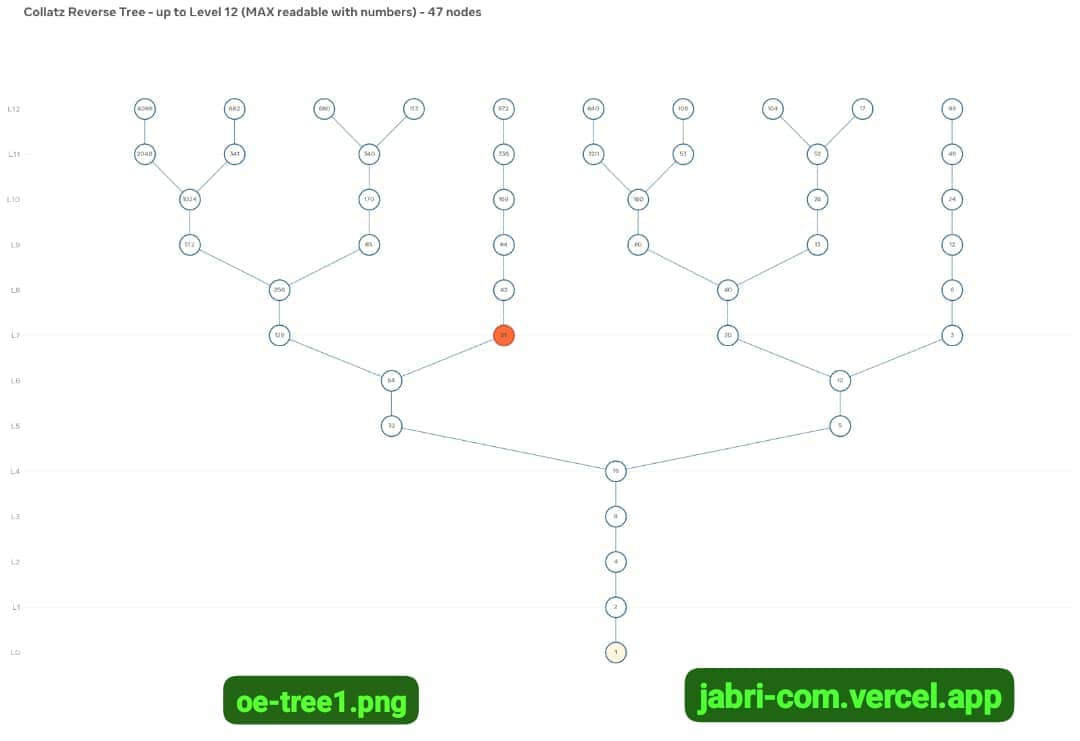
\includegraphics[width=0.9\textwidth]{oe-tree1.png}
\\[4pt]
\small \textbf{الشكل 1:} رسمتك اليدوية بعد التحويل الرقمي \\
\small $1 \to 2 \to 4 \to 8 \to 16 \to 5 \to 10 \to 3$
\end{center}

\begin{center}
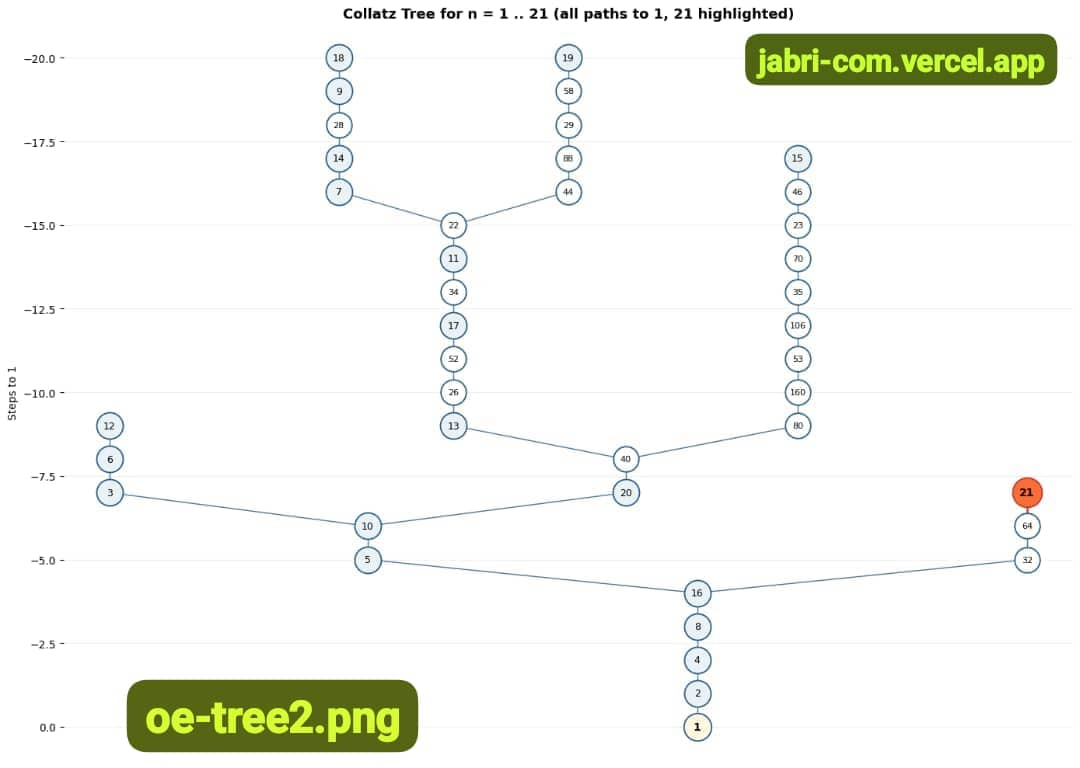
\includegraphics[width=0.9\textwidth]{oe-tree2.png}
\\[4pt]
\small \textbf{الشكل 2:} oe-tree2.png
\end{center}

\begin{center}
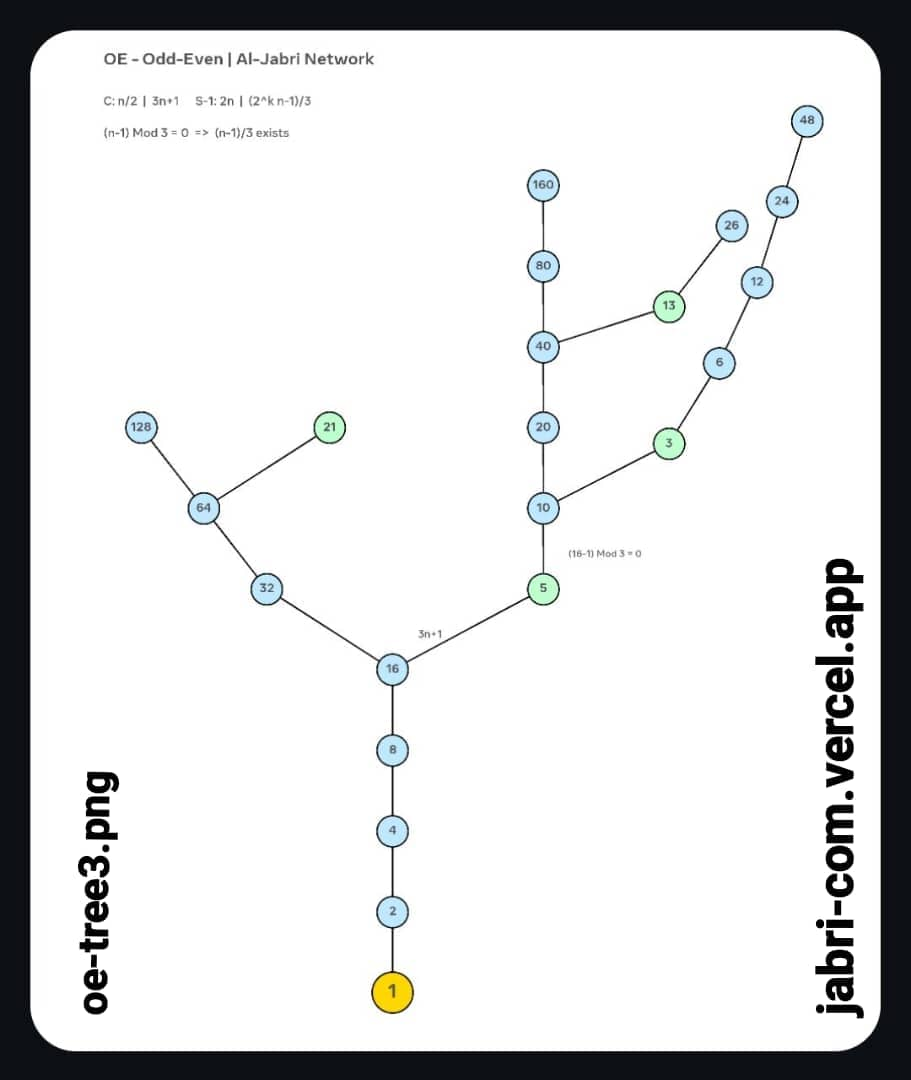
\includegraphics[width=0.9\textwidth]{oe-tree3.png}
\\[4pt]
\small \textbf{الشكل 3:} oe-tree3.png
\end{center}

\begin{center}
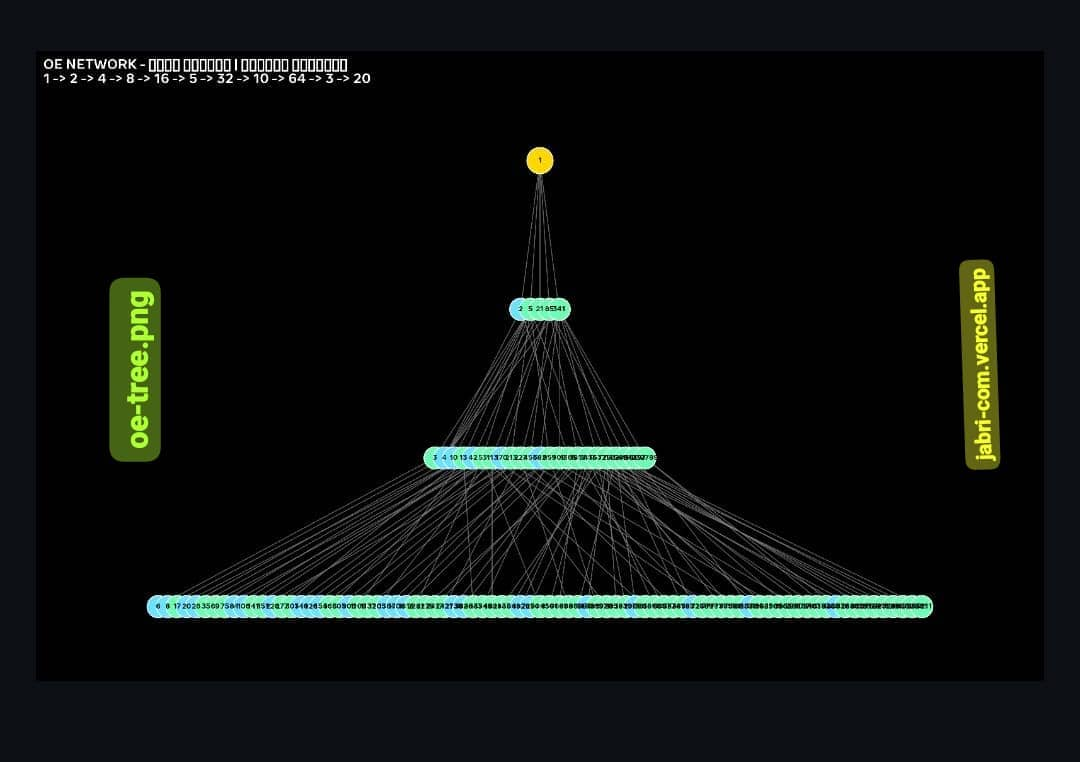
\includegraphics[width=0.9\textwidth]{oe-tree.png}
\\[4pt]
\small \textbf{الشكل 4:} الشبكة الكاملة - oe-tree.png
\end{center}

\begin{center}
\small
$Z + C + A = 1$ --- الزوجي + الفردي + الشبكة = الواحد الأحد \\
\textenglish{Odd-Even --- OE}
\end{center}

% ===== فوتر نهاية المستند - مثل footer.html =====
\vspace{1cm}
\begin{center}
\rule{0.8\textwidth}{0.4pt} \\
\small \textbf{م/ عبدالله محمد ناصر الجبري} \\
\small تعز - الجمهورية اليمنية | \textenglish{jabri62018@gmail.com} | \textenglish{ORCID: 0009-0003-3319-3822} \\
\small \textenglish{jabri-com.vercel.app} | \textenglish{@jabri2025} \\
\small \textenglish{Sinbad Unified Theory: Z + C + A = 1} \\
\small \textenglish{© 2026 Abdulla Mohammed Nasser Al-Jabri — All Rights Reserved} \\
\small الزوجي والفردي --- OE --- \today
\end{center}

\end{document}